\chapter{State of the Art}
Innerhalb der nächsten Seiten wird die vorliegende Arbeit in den aktuellen Stand der Forschung eingeordnet.
Zu diesem Zweck werden aktuelle Arbeiten in Bezug auf die Anwendung und Anwendbarkeit von Brain Computer Interfaces vorgestellt.\\


\section{Aktuelle BCI-Anwendungen}
Die nachfolgenden Artikel beschreiben einige BCI-Anwendungen aktueller Forschungen unter Verwendung verschiedener Brain Computer Interfaces und den zugrunde liegenden Paradigmen.\\

\subsection{Brain Chess}
\vspace{0.3cm}
\label{chessconcept}
Schach ist ein rundenbasiertes Denkspiel, das durch seinen Aufbau und durch seinen vergleichweise langsamen Spielablauf hervorragend für eine \acs{BCI}-Steuerung geeignet ist.
"`Brain Chess – Playing Chess using Brain Computer Interface"' \cite[S.1-5]{BCIChess} befasst sich mit der Konzeption eines Schach-Spiels gesteuert durch ein Brain Computer Interface.
Vorranging werden in diesem Artikel Möglichkeiten erörtert, wie eine Steuerung einzelner Spielabschnitte unter Verwendung von Gehirnsignalen realisiert werden könnte.\\


Um eine Schachfigur auszuwählen muss zunächst mit Hilfe von einem Trainingsdatensatz, der spezifische Signalwert einer Figur ermittelt werden.
Dies wird durch ein "`Memory Card Game"' realisiert, so dass für jede Figur ein durchnittlicher Wert berechnet werden kann.
Anhand dieses Werts kann im Spielverlauf eindeutig bestimmt werden, welche Art von Figur ausgewählt wurde.\\

Sobald die Art der Figur bekannt ist, kann diese im Rahmen ihrer Möglichkeiten bewegt werden. 
Um die Bewegung zu realisieren wird eine Steuerung auf Basis von sensomotorischer Rhythmen (\acs{SMR}) vorgeschlagen, da dies die Unterscheidung einiger weniger Aktionen ermöglicht.
So können mit Hilfe der Vorstellung von Hand- oder Fußbewegungen die Bewegung der Schachfigur, wie in Abbildung\footnote[1]{Bild-Quelle: \cite[S.4]{BCIChess}} \ref{ChessPawn}, bestimmt werden.\\

\begin{figure}[h!]
\begin{center}
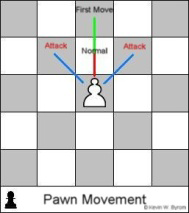
\includegraphics[scale=0.6]{images/ChessPawn.png}
\caption{Die vier Bewegungsmöglichkeiten eines Bauern, welche mit der Vorstellung von Hand- und Fußbewegungen assoziert werden können}
\label{ChessPawn}
\end{center}
\end{figure}

\begin{figure}[h!]
\begin{center}
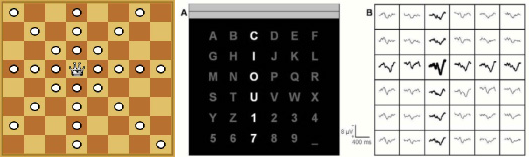
\includegraphics[scale=0.7]{images/QueenControlExample.png}
\caption{Die Bewegungsmöglichkeiten einer Dame deren Zielfeld mit einem P300-Speller ausgewählt werden könnte}
\label{ChessQueen}
\end{center}
\end{figure}

Dies funktioniert allerdings nicht für jede Schachfigur.
Denn eine Dame, ein Läufer und ein Turm können sich nicht nur in verschiedene Richtungen bewegen, sondern auch unterschiedlich weit.
Für diese Steuerung wird eine dem P300-Speller nahe kommende Methode wie in Abbildung\footnote[2]{Bild-Quelle: \cite[S.5]{BCIChess}} \ref{ChessQueen} vorgeschlagen, so dass das Zielfeld auf Basis einer 8x8-Matrix genau ausgewählt werden kann.








\pagebreak
\subsection{Design und Implementierung eines BCI-Schachs}
\label{chessDesignAndImplemention}
Der Artikel \cite{toersche2007designing} befasst sich ebenfalls mit dem Design und der Implementierung einer BCI-Steuerung für Schach.
Dafür werden zunächst die Rahmenbedingungen festgelegt, sodass ein quelloffenes Schach-Spiel und die \acs{BCI2000}-Plattform für die BCI-Steuerung verwendet werden soll.
Die Steuerung soll über einen P300-Speller erfolgen.
In diesem Zusammenhang wird sich mit der Art der Stimuli auseinandergesetzt, ob diese durch Zeilen und Spalten oder einzelne Zellen des Schachbretts dargestellt werden.
Ein P300-Speller der Zellen hervorhebt, kann das Problem haben, dass nicht genügend Zellen zur Verfügung stehen, sodass leere Zellen zur Auswahl hinzugefügt werden müssen.
Dieses Problem tritt beim Zeilen-/Spalten-Speller nicht auf, weshalb ihm der Vorzug zu gewähren ist.
Insbesondere weil die Genauigkeit weiter erhöht werden kann, 
indem nicht erreichbare Zeilen in einigen Spielabschnitten als Ergebnis ausgeschlossen werden können.\\
Ein wichtiger Aspekt auf den das Design eingeht, ist die individuell benötigte Zeit zum Nachdenken.
Da jedem Zug eine gewisse Zeit zum Denken vorausgeht, werden einige Möglichkeiten betrachtet, um dieses Problem zu lösen.
Würde pauschal eine gewisse Zeit zur Verfügung gestellt werden, kann diese in der einen Runde zu viel und in der anderen zu wenig sein.
Ein Lösungsvorschlag dieses Problems ist die Verwendung eines weiteren BCIs, das bei einer imaginären Handbewegung den Zug beginnt, jedoch wird dadurch die Komplexität erhöht.
Alternativ und damit weniger komplex wird diese Option in den Speller integriert, sodass die Auswahl eines unbesetzten Feldes die Denkzeit erhöht.
Für eine eventuelle Implementierung mit einem Zellen-Speller würde einfach eine Zelle außerhalb des Schachbretts dargestellt, deren Auswahl ebenfalls die Denkzeit erhöht.\\
Im weiteren Verlauf wird das Design der Implementierung vervollständigt, sodass die Kommunikation zwischen zwei Spielern über einen Server mittels IRC durchgeführt wird.
Die BCI2000-Plattform kommuniziert über eine Schnittstelle für externe Anwendungen mit einem BCI-Schach-Logik-Modul (BSLM), 
das alle Komponenten miteinander verknüpft, sodass die Signale des BCI vom BCI2000 empfangen und verarbeitet werden.
Die weitere Verarbeitung und Darstellung der Stimuli erfolgt durch das BSLM und das Schachspiel.\\
Abschließend befasst sich die Studie mit einer Analyse der Genauigkeit und der benötigten Zeit pro Zug.
Zu diesem Zeitpunkt ist die Implementierung des Schachspiels jedoch noch nicht abgeschlossen, weshalb die Genauigkeit und die benötigte Zeit nur theoretisch, anhand bestehender Daten anderer Quellen, errechnet wird.\\








\pagebreak
\subsection{Manuelle BCI-Steuerung eines Rollstuhls}
\vspace{0.3cm}

Die Steuerung eines Rollstuhls per \acs{BCI} ist eine erstrebenswerte Anwendung für Patienten mit motorischen Störungen.
\ac{LIS}-Patienten würden auf diese Weise ein gewisses Maß an Eigenständigkeit zurückerlangen und ihre Hilfsbedürftigkeit verringern.
Mit diesem Thema befassen sich deshalb zwei wissenschaftliche Studien (Studie 1 \cite{wheelchairBCI2}, Studie 2 \cite{wheelchairBCI3}), die in den nächsten Seiten genauer betrachtet werden.\\



Beide Studien verwendeten in ihrer Arbeit ein kombiniertes System bestehend aus BCI-Gerät, 
das anhand von mentalen Aufgaben (motorisch und kognitiv) gesteuert wurde und einem intelligentem Rollstuhl, der mit Hilfe eines Lasers die Umgebung abtastete.
Ein Hindernis links vom Rollstuhl bewirkte eine Einschränkung der Bewegungsmöglichkeiten, so dass der Befehl "`Turn Left"' eine Wahrscheinlichkeit von 0\% erhielt.
In den Experimenten beider Studien assoziierte jede Testperson einen Steuerbefehl ("`Turn Left"', "`Forward"' und "`Turn Right"') mit einer mentalen Aufgabe.
Das BCI wertete 16 EEG-Muster pro Sekunde aus und lieferte alle 0,5 Sekunden einen Befehl für den Rollstuhl.
Im der ersten Studie bekamen zwei Testpersonen die Aufgabe in zehn Versuchen 
und in fünf Sitzungen einen vordefinierten Weg in einer virtuellen Umgebung (siehe Abbildung\footnote[1]{Bild-Quelle: \cite[S.2161]{wheelchairBCI2}} \ref{TestEnvWheelchair}) zurückzulegen.\\

\begin{figure}[h!]
\begin{center}
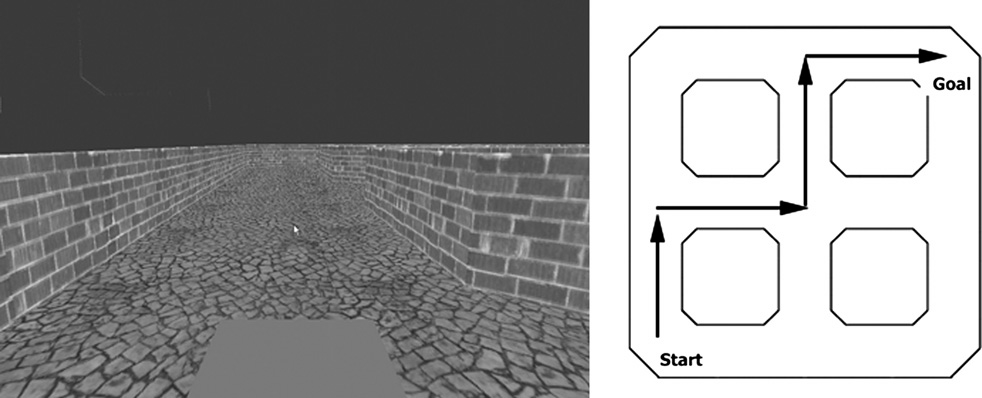
\includegraphics[scale=0.45]{images/TestEnvWheelchair.png}
\caption{Die virtuelle Rollstuhlumgebung und der zu absolvierende Weg.}
\label{TestEnvWheelchair}
\end{center}
\end{figure}

Die erreichten Ziele variierten von 40-100\% und von 10-80\% bei den beiden Testpersonen, wobei die niedrigen Werte am Anfang (40\%, 10\%) mit einem Lernprozess begründet werden. 
Im Vergleich dazu erreichten nur 1\% von 100 zufallsgesteuerten Versuchen innerhalb der Versuchsdauer das Ziel. \\

Darauf aufbauend wurde in der zweiten Studie ein ähnliches Experiment in der realen Welt durchgeführt.
Zusätzlich zu den bisherigen EEG-Daten wurden \ac{EMG}- und \ac{EOG}-Daten erfasst um auszuschließen, 
dass Augenbewegungen oder Muskelaktivität im EEG-Signal fälschlicherweise als Kontrollsignale gewertet werden.\\

In diesem Experiment bestand die Aufgabe darin, auf einem Weg drei Ziele nacheinander zu passieren.
Gemessen wurde dabei wie nah jede Testperson den Zielen bei jedem Versuch kam.
Dem wurde wieder ein Zufallsgesteuertes BCI gegenübergestellt. 
In Abbildung\footnote[1]{Bild-Quelle: \cite[S.8]{wheelchairBCI3}} \ref{WheelchairResults} ist zu sehen, wie weit die einzelnen Testsubjekte bzw. das zufallsgesteuerte BCI vom Ziel entfernt waren.\\

\begin{figure}[h!]
\begin{center}
\includegraphics[scale=0.85]{images/WheelchairResults2.png}
\caption{Testergebnisse des Experiments aus Studie 2. Die zurückgelegte Dis\-tanz ist auf der X-Achse und die prozentual erreichten Ziele auf der Y-Achse abgebildet.}
\label{WheelchairResults}
\end{center}
\end{figure}


Die Ergebnisse zeigten wie schon in der ersten Studie, dass die Personen in der Lage waren einen Rollstuhl in Echtzeit zu kontrollieren 
und damit eine Aufgabe, die schnelle und genaue Entscheidungen abverlangt, zu bewältigen. 
Die Ergebnisse des ersten Experiments in der virtuellen Umgebung schnitten dabei jedoch besser ab als die in der realen Welt, obwohl beide noch weit vom Optimum entfernt sind.











\pagebreak
\subsection{P300-Steuerung eines Rollstuhls mit automatischer Navigation}
\vspace{0.3cm}

Für die Steuerung eines Rollstuhls betrachtet die Studie \textit{"`Synchronous EEG Brain-Actuated Wheelchair with Automated Navigation"'} \cite{WheelchairBCI1} einen anderen Ansatz.
In diesem wird lediglich die Auswahl des Ziels vom Rollstuhlfahrer übernommen, so dass nach Eingabe ein automatisches Navigationssystem den Rollstuhl an sein Ziel steuert.
Für diese Anwendung wurden in einem herkömmlichen elektrischen Rollstuhl zwei Computer verbaut, die für die Motorsteuerung und für die Berechnung der Navigation zuständig waren.
Der Fahrer des Rollstuhls hatte zusätzlich einen Notebook vor sich, über den die visuelle Stimuli-Präsenation durchgeführt wurde. 
Darüber hinaus war der Rollstuhl auch mit einem Laser ausgestattet, sodass Hindernisse in der Navigation und Zielauswahl berücksichtigt werden konnten.
Für die Zielauswahl wurde eine grafische Benutzeroberfläche verwendet, die eine vereinfachte virtuelle Ansicht der Benutzerwahrnehmung darstellte.
Auf der Benutzeroberfläche wurde unter Verwendung des P300-Paradigmas eine Matrix bzw. ein Gitter, wie in Abbildung\footnote[1]{Bild-Quelle: \cite[S.2]{WheelchairBCI1}} \ref{WheelchairGUI} zu sehen, mit vier Zeilen und fünf Spalten dargestellt. 
Die ersten drei Zeilen entsprachen den Zielen und staffelten sich in 8m, 4m und 2m Abständen.
Die fünf Spalten entsprachen jeweils einem Winkel von -60°, -30°, 0°, 30° und 60°.\\

\begin{figure}[h!]
\begin{center}
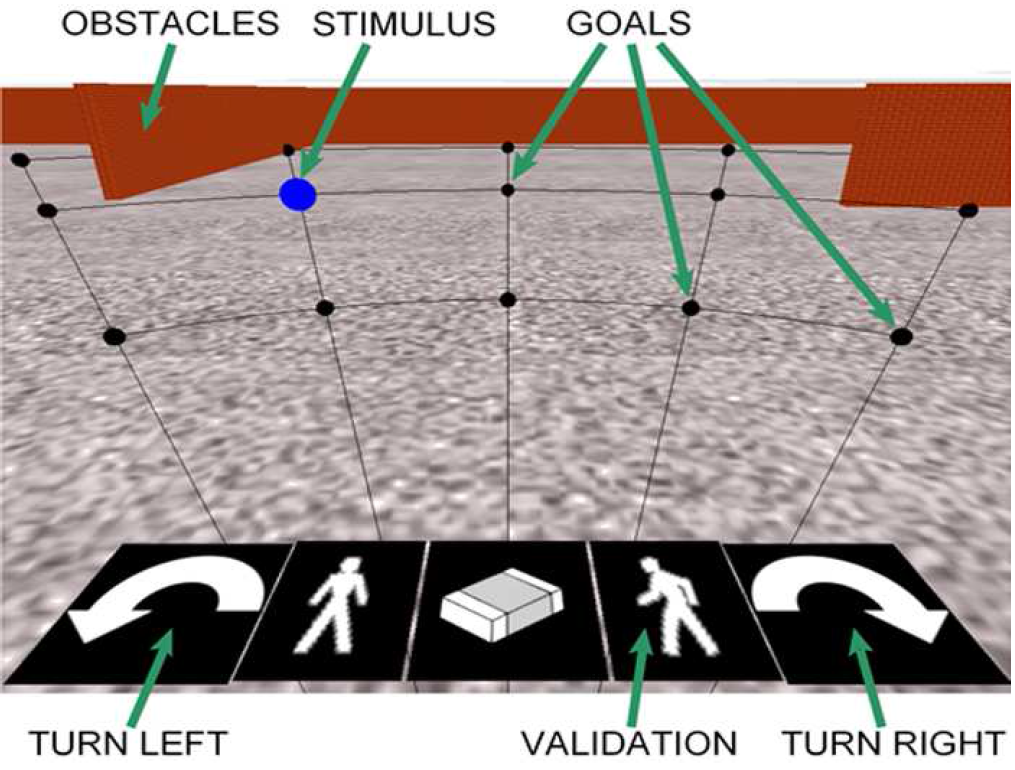
\includegraphics[scale=0.32]{images/WheelchairGUI.png}
\caption{Die grafische Benutzeroberfläche für die Zielauswahl des Rollstuhls.}
\label{WheelchairGUI}
\end{center}
\end{figure}

\pagebreak
Jede Zielauswahl erfolgte in zwei Schritten. Zunächst wurden die Stimuli-Sequenzen abgespielt, sodass ein Zielpunkt ausgewählt werden konnte.
Anschließend musste dieser entweder bestätigt werden, indem das Validierungssymbol ausgewählt wurde 
oder es konnte Schritt eins wiederholt und ein neuer Zielpunkt ausgewählt werden.
Bei erfolgreicher Zieleingabe übernahm das Navigationssystem die Kontrolle, während die BCI-Steuerung in einem Wartezustand verblieb, bis das Ziel erreicht wurde.
Um an das endgültige Ziel zu gelangen waren mitunter mehrere Zwischenziele nötig, sodass die Kontrolle immer zwischen BCI-Steuerung und Navigationsystem wechselte.\\

Das System wurde in einem Experiment mit fünf gesunden männlichen Testpersonen durchgeführt und wurde in drei Phasen unterteilt, die ersten beiden dienten der Unterweisung und dem Training der Testpersonen. 
In der dritten Phase mussten jeweils zwei vordefinierte Routen absolviert werden. 
Dies wurde von allen Testpersonen erfolgreich abgeschlossen.
Die erzielte durchschnittliche Genauigkeit der BCI-Steuerung entsprach während dieser Phase 94\% und zeigt somit eine gute Anwendbarkeit des Systems.\\










\pagebreak
\subsection{Steuerung eines Pinball-Spielautomaten}
\vspace{0.3cm}

Die Studie \textit{"`Playing Pinball with non-invasive BCI"'} \cite{BCIPinball} befasst sich mit der Steuerung eines Pinball-Spielautomaten in Echtzeit.
Für dieses Experiment wurde der Automat präpariert, sodass die Spielbälle ausschließlich an den beiden Kontroll-Paddeln vorbei konnten 
und das Gefälle des Automaten wurde etwas verringert, um das Spiel zu verlangsamen.
Die Steuerung erfolgte unter Verwendung von sensomotorischen Rhythmen. Die Vorstellung einer linken bzw. rechten Handbewegung steuerte die jeweiligen Kontroll-Paddel.
Für die Tests wurden bereits erfahrene BCI-Testpersonen verwendet. Allerdings erreichten nicht alle eine verlässliche Kontrolle über das Spiel, sodass diese von der Bewertung ausgeschlossen wurden.
Alle 0,5 Sekunden wurden die EEG-Daten ausgewertet und in einen Befehl übersetzt. Die Ergebnisse wurden aufgezeichnet und den Ergebnissen einer Pseudo-Zufallssteuerung gegenübergestellt.
Die Qualität der einzelnen Bälle, 
sowie deren Dauer und die Gesamtpunktzahl der Testpersonen war deutlich besser als die der Pseudo-Zufalls-Kontrolle (siehe Abbildung\footnote[1]{Bild-Quelle: \cite[S.7]{BCIPinball}} \ref{PinballBCI}).\\

\begin{figure}[h!]
\begin{center}
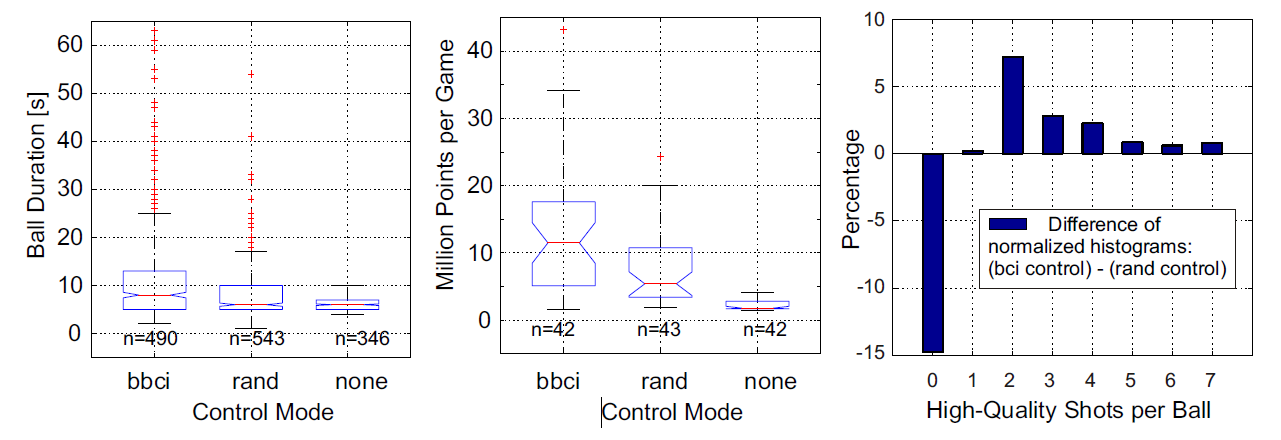
\includegraphics[scale=0.45]{images/PinballBCI.png}
\caption{Die durchschnittlichen Ergebnisse der vier bewerteten Testsubjekte im Vergleich zu den Ergebnissen der Pseudo-Zufalls-Kontrolle, sowie den Ergebnissen, die ohne jede Kontrolleinwirkung erzielt wurden.}
\label{PinballBCI}
\end{center}
\end{figure}

Es zeigt sich damit, dass die Kontrolle eines stark modifizierten Pinball-Spielautomaten in Echtzeit durch ein Brain Computer Interface möglich ist. \\











\pagebreak
\subsection{Stimuli-Präsentation nicht-statischer Objekte}
\vspace{0.3cm}
Das am häufigsten verwendete \acs{BCI} basiert auf dem P300 Paradigma. In den meisten Fällen wird bei den verwendeten BCIs die Stimulation visuell erzeugt.
In äquidistanten Zeitabständen werden Objekte gleichverteilt und in zufälliger Reihenfolge auf dem Bildschirm hervorgehoben.
Dies funktioniert mit vielen Geräten relativ gut, sofern diese über statische Bedienelemente verfügen. 
Bei interaktiven Szenerien stößt dieser Ablauf allerdings an seine Grenzen,
denn beispielsweise sind in Computerspielen sich bewegende Elemente ein signifikanter Bestandteil.\\

Im Rahmen der Studie 
\textit{"`A P300-based Brain-Computer Interface with Stimuli on Moving Objects: Four-Session Single-Trial and Triple-Trial Tests with a Game-Like Task Design"'} 
\cite[S.5ff]{P300Moving} wurde ein experimentelles Spiel erstellt.


\begin{figure}[h!]
\begin{center}
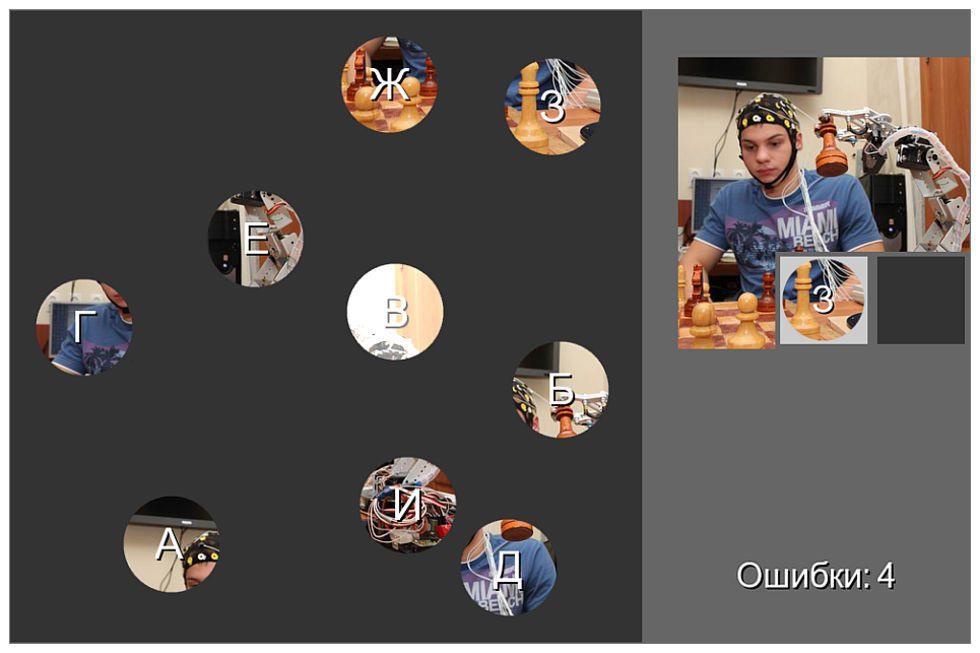
\includegraphics[scale=0.33]{images/MovingStimuliPuzzle.png}
\caption{Die Puzzleteile mit hervorgehobenem Kreis "`B"' und dem bisher zusammengesetzten Puzzle}
\label{MovingStimuliPuzzle}
\end{center}
\end{figure}

Das Ziel des Spiels war, ein Puzzle aus neun Bildfragmenten zusammen zu bauen.
Alle Puzzleteile wurden in gekennzeichneten Kreisen wie in Abbildung\footnote[1]{Bild-Quelle: \cite[S.8]{P300Moving}} \ref{MovingStimuliPuzzle} zu sehen, vor einer schwarzen Fläche angezeigt.
Aus den Kennzeichnungen ergab sich eine alphabetische Reihenfolge, woran sich die Spieler orientieren mussten.
Sobald das Spiel gestartet wurde, bewegten sich die Kreise in zunächst zufällige Richtungen, 
welche im weiteren Verlauf von Kollisionen mit anderen Kreisen oder dem Außenrand beeinflusst wurden.
Die Kreise wurden während sie sich bewegten in zufälliger Reihenfolge hervorgehoben.\pagebreak

Die Aufgabe jedes Spielers war es den Kreis der aktuellen Kennzeichnung zu fokussieren, 
diesen zu verfolgen und sich darauf zu konzentrieren, ob oder wie oft der Kreis aufblitzte.\\
Die Teilnehmer dieses Experiments wurden darüberhinaus in zwei Gruppen aufgeteilt.
Einer Gruppe "`Single-Trial"' wurden pro Durchlauf alle Kreise nur jeweils ein mal hervorgehoben, der anderen "`Triple-Trial"' hingegen jeweils drei mal.
Bei einer falschen Auswahl wurde dem Spieler ein Fehlerpunkt hinzuaddiert. Erreichte ein Spieler zehn Fehlerpunkte, so hatte er das Spiel verloren.
Gewonnen wurde das Spiel, sobald das Puzzle vollständig war.\\

Die Durchführung dieser Tests zeigte auf, dass die Genauigkeit der Ergebnisse beim "`Single-Trial"' geringer war als bei der "`Triple-Trial"'-Gruppe, 
im Umkehrschluss war jedoch das Interesse am Spiel bei der "`Single-Trial"'-Gruppe größer, da ein höherer Spielfluss stattfand.
Das Experiment zeigte, dass das P300 Paradigma sich permanent bewegende Objekte registrieren kann \cite[S12]{P300Moving} und diese Art der Stimuli-Präsentation reale Anwendung finden kann. 
Mit höherem Spielfluss bzw. höherer Geschwindigkeit muss allerdings ein Verlust an Genauigkeit in Kauf genommen werden.\\











\pagebreak
\subsection{Ein auf P300 basierendes haptisches \acs{BCI}}
\vspace{0.3cm}
% Mit Hilfe des \acs{P300 ERP} kann einem Menschen mit dem sogenannten \ac{LIS} eine Möglichkeit gegeben werden, mit seiner Umwelt zu kommunizieren.
% Patienten mit \acs{LIS} sind in ihrem Körper gefangen, sie verfügen nicht über die Möglichkeit der Selbstdarstellung, obwohl sie bei vollem Bewusstsein sind.
% Viele aktuelle \acs{BCI} Anwendungen ermöglichen Kommunikation, indem sie \acs{P300 ERP}'s evozieren.

Bei einer Person mit einem eingeschränkten Bewusstsein bzw. ohne ein mindestmaß an visueller Wahrnehmung, ist eine visuelle Stimulation und eine darauf basierende Kommunikation nicht möglich.
Unabhängig davon verfügen viele betroffene Menschen weiterhin über ihren Tastsinn.\\
In der Studie \textit{"`A Tactile P300-Based BCI"'} \cite[Art. 98]{P300Tactile} wurde ein auf dem Tastsinn und dem \acs{P300 ERP} basierendes \acs{BCI} präsentiert.
Dieses ermöglicht einer Person die Kommunikation mittels haptischer Stimulation.
Hierfür wurden drei Szenarien getestet, in denen die Stimuli repräsentiert durch kurze Vibrationen einen \acs{P300 ERP} evozierten.\\

\begin{itemize}

\item[\textbf{Szenario 1: }] Den Testpersonen wurden jeweils zwei Stimulatoren an die Handgelenke angelegt. 
Einer der Stimulatoren vibrierte in regelmäßigen, der andere in unregelmäßigen Abständen. 
Wenn sich die Testpersonen auf die unregelmäßigen Vibrationen konzentrierten, löste dies zuverlässig ein \acs{P300 ERP} aus.

\item[\textbf{Szenario 2: }] In diesem Szenario wurden drei Stimulatoren verwendet, der dritte befindet sich hierbei auf dem Rücken und vibriert in regelmäßigen Abständen.
Auf diese Weise ist es möglich, mit den beiden Stimulatoren an den Handgelenken, einfache Ja/Nein-Antworten zu erzeugen.

\item[\textbf{Szenario 3: }] Im dritten Szenario wurden die Hände der Probanden mit vier Stimulatoren, jeweils einem pro Finger mit Ausnahme des Daumens versehen.
Jeder dieser Stimulatoren wurde mit gleicher Wahrscheinlichkeit zum vibrieren gebracht.
Die Testpersonen mussten sich in jedem Testlauf in zufälliger Reihenfolge auf einen Finger konzentrieren,
so dass für jeden Finger ein \acs{P300 ERP} erzeugt wurde.\\
\end{itemize}

Die mittlere Genauigkeit aller Probanden der drei Szenarien lag bei 100\%, 80\% und 69,4\%.






\pagebreak
\section{Einordnung in den State of the Art}

Diese Masterarbeit lässt sich im Vergleich zu den meisten behandelten Studien nicht eindeutig einordnen.
Im Bereich der Konzeption einer BCI-Anwendung ist sie vergleichbar mit der Studie "`Brain Chess – Playing Chess using Brain Computer Interface"' von Seite \pageref{chessconcept}, 
allerdings behandelt diese Studie nur die theoretischen Realisierungsmöglichkeiten und kann keine Implementierung vorweisen.\\

Einen Schritt weiter ist die darauf folgende Studie auf Seite \pageref{chessDesignAndImplemention}, diese befasst sich zwar auch weitestgehend mit der Planung eines Schachspiels, 
jedoch wird das Gesamtkonzept tiefergehend betrachtet. 
Hierzu gehört die Verknüpfung der \acs{BCI2000}-Plattform und dem Spiel durch ein BCI-Schach-Logik-Modul als Schnittstelle.
Diese Masterarbeit lässt sich daher im Bereich dieser Studie einordnen, da diese ebenso eine Möglichkeit zur Steuerung eines Spiels plant und realisiert.\\

Alle weiteren Studien befassen sich ebenfalls mit möglichen BCI-Anwendungen, insbesondere mit einigen Anwendungen des \acs{P300 ERP}, 
allerdings sind diese mehr auf die Ergebnisse der jeweiligen Experimente fokussiert und beschreiben weniger die Implementierungsmöglichkeiten für vergleichbare BCI-Erweiterungen.
Die Genauigkeit ist darüberhinaus bei allen Studien ein wichtiger Betrachtungspunkt. 
In Bezug auf diese Arbeit kann daher vorallem eine Balance zwischen Genauigkeit und Spielfluss erforderlich sein, 
da ein zu langsamer Spielfluss möglicherweise die Aufmerksamkeit und damit die Genauigkeit verschlechtern könnte.\\






















